\documentclass[conference]{IEEEtran}
\IEEEoverridecommandlockouts
\usepackage{cite}
\usepackage{amsmath,amssymb,amsfonts}
\usepackage{graphicx}
\usepackage{booktabs}
\usepackage{array}
\usepackage{xcolor}
\usepackage{url}
\usepackage{tikz}
\usetikzlibrary{arrows.meta,positioning,shapes.geometric,fit,calc,backgrounds}

% "\pend" marks a number that the v2 notebook fills in (tables/*.tex). None should remain at submission.
\newcommand{\pend}{\textcolor{red}{\textbf{[run]}}}
\newcommand{\aucTabAS}{0.583}
\newcommand{\aucTabASV}{0.737}
\newcommand{\aucImage}{0.887}
\newcommand{\aucFusAS}{0.884}
\newcommand{\aucFusASV}{0.884}
\newcommand{\dAucFusAS}{-0.0025}
\newcommand{\dAucFusASlo}{-0.0088}
\newcommand{\dAucFusAShi}{+0.0035}
\newcommand{\pFusAS}{=0.368}
\newcommand{\dAucFusASV}{-0.0027}
\newcommand{\dAucFusASVlo}{-0.0075}
\newcommand{\dAucFusASVhi}{+0.0021}
\newcommand{\pFusASV}{=0.279}
\newcommand{\seedDAucFusAS}{-0.0004}
\newcommand{\seedDAucFusASsd}{0.0038}
\newcommand{\seedDAucFusASV}{-0.0020}
\newcommand{\seedDAucFusASVsd}{0.0038}
\newcommand{\seedSigFusAS}{1}
\newcommand{\seedSigFusASV}{1}
\newcommand{\shareFusAS}{0.98}
\newcommand{\shareFusASV}{1.50}
\newcommand{\shareFusASVap}{1.97}
\newcommand{\shareFusASVpa}{1.09}
\newcommand{\energyImage}{0.244}
\newcommand{\energyChance}{0.123}
\newcommand{\pointImage}{0.454}
\newcommand{\nLoc}{1082}
\newcommand{\cramersV}{0.36}
\newcommand{\nTest}{4404}
\newcommand{\nTrain}{20401}
\newcommand{\nVal}{4879}
\newcommand{\extAucAImage}{0.781}
\newcommand{\extAucAFusAS}{0.745}
\newcommand{\extAucAFusASV}{0.770}
\newcommand{\extAucATabASV}{0.577}
\newcommand{\extNA}{6145}
\newcommand{\extPosA}{145}
\newcommand{\extAucBImage}{0.675}
\newcommand{\extAucBFusAS}{0.656}
\newcommand{\extAucBFusASV}{0.687}
\newcommand{\extAucBTabASV}{0.550}
\newcommand{\extNB}{8812}
\newcommand{\extPosB}{2812}
% Table rows are read with the TeX primitive so they work inside tabular
\makeatletter\newcommand{\inputrows}[1]{\@@input #1 }\makeatother
% Include a figure if the file exists, otherwise draw a placeholder box (so the draft always compiles)
\newcommand{\figfile}[2]{\IfFileExists{figures/#1}{\includegraphics[width=#2]{figures/#1}}{\fbox{\parbox{#2}{\centering\vspace{1.2cm}\textcolor{red}{figure \texttt{#1} -- copy from Kaggle output}\vspace{1.2cm}}}}}

\begin{document}

\title{Explainable Multimodal Pneumonia Detection on Chest Radiographs: Does Patient Metadata Help?}

\author{
\IEEEauthorblockN{Fatima Siddiqa}
\IEEEauthorblockA{Roll No. 23i-2543\\
Department of Data Science,FAST University\\
Islamabad, Pakistan}
\and
\IEEEauthorblockN{Mariam Shaiq}
\IEEEauthorblockA{Roll No. 23i-3250\\
Department of Data Science, FAST University\\
Islamabad, Pakistan}
}

\maketitle

% ======================================================================
\begin{abstract}
Multimodal models that fuse chest radiographs with patient data are often reported to outperform image-only models, yet it is rarely checked \emph{which} modality drives a prediction or whether the gain comes from clinically irrelevant cues. We address this for pneumonia detection on the RSNA Pneumonia Detection Challenge data (29,684 radiographs, 12,233 patients) linked to NIH ChestX-ray14 metadata. We trained a DenseNet-121 image-only base model and two nested intermediate-fusion extensions that add age and sex, and then also view position. We evaluated them with patient-level bootstrap confidence intervals, DeLong tests, three training seeds, subgroup analyses, an occlusion-based modality-contribution measure adopted from our base paper, and Grad-CAM localisation against 11,390 radiologist boxes; external validation used held-out NIH images. View position alone separated the classes well (metadata-only AUC \aucTabASV\ vs.\ \aucTabAS\ without it; Cram\'er's $V=\cramersV$), but this advantage fell to \extAucATabASV\ on the external data, confirming view as a site-specific shortcut. The image-only model reached an AUC of \aucImage. Adding age and sex gave \aucFusAS\ ($\Delta$AUC $\dAucFusAS$, 95\% CI $[\dAucFusASlo, \dAucFusAShi]$), and adding view gave \aucFusASV; across three seeds the mean gain was $\seedDAucFusAS$, so fusion did not improve performance. Occlusion showed that metadata accounted for only \shareFusAS\%--\shareFusASV\% of the prediction change, and Grad-CAM placed \energyImage\ of its mass inside expert boxes, about twice the chance level of \energyChance. On the external set all models lost accuracy (image-only AUC \extAucAImage\ for pneumonia), and no fusion model was consistently better. Fusing basic demographics thus added nothing measurable, and the audit pipeline we release makes such null results, and possible shortcuts, visible.
\end{abstract}

\begin{IEEEkeywords}
multimodal deep learning, explainable AI, pneumonia detection, chest radiograph, shortcut learning, modality contribution
\end{IEEEkeywords}

% ======================================================================
\section{Introduction}
\label{sec:intro}

Deep convolutional networks now detect pneumonia and other thoracic findings on chest radiographs at a level comparable to radiologists~\cite{rajpurkar2018chexnext}. Clinicians, however, do not read an image in isolation: they take into account the patient's age, sex and the context of the examination when interpreting a finding. This has led to the development of multimodal models that combine the image with the associated structured patient data, which has been reported to improve performance on a range of clinical tasks.~\cite{soenksen2022haim,acosta2022multimodal}.

Two problems limit what these gains mean. Firstly, a higher ROC curve (AUC) does not show \emph{why} the model has improved. The data may be predictive in a statistical sense but not necessarily in a medical one. A classic example on chest X-rays is the difference between anteroposterior (AP) and posteroanterior (PA) films. AP films are taken with the portable unit in the patient's room as the patient is too unwell to stand, while PA films are taken in the radiology department~\cite{zech2018confounding}. A model that learns "AP = sick" can do very well and yet still fail when the case mix of the hospital changes; this is the phenomenon of shortcut learning~\cite{geirhos2020shortcut,degrave2021shortcuts}. Secondly, explanation tools such as Grad-CAM~\cite{selvaraju2017gradcam} show where the image model is looking but nothing about the contribution of the non-image inputs. Gapp \emph{et al.}~\cite{gapp2025modality}'s paper, which is the base paper of this study, tackled the second issue by proposing an occlusion based measure of the contribution of each modality to the output of a multimodal model. 


\textbf{Research gap.} The base paper quantifies modality contribution. However, the contribution of different modalities is not assessed to determine if it can be considered a shortcut, and no image level localisation is provided with expert annotations. While fusion methods for x-ray images~\cite{truong2025multimodal,soenksen2022haim} improve accuracy, signal and noise cannot be separated. In saliency methods~\cite{saporta2022saliency,arun2021trustworthiness}, image explanation is assessed without considering other modalities. 

\textbf{Novelty.} We combine the base paper's modality-contribution measure with a deliberately nested model design in which a known shortcut variable (view position) is added in a controlled step. This turns the contribution measure into a test: if fusion relies on the shortcut, the measure and the view-stratified performance should reveal it. We also evaluate Grad-CAM against radiologist bounding boxes in the same models and validate on a second, external dataset.

\textbf{Contributions.}
\begin{enumerate}
\item We build and release a reproducible linkage of 29,684 RSNA radiographs to NIH metadata with a patient-level split, and show that view position is strongly associated with the label (Cram\'er's $V=\cramersV$; metadata-only AUC rises from \aucTabAS\ to \aucTabASV\ when view is added).
\item We compare an image-only base model with two nested fusion models using 5,000-resample patient-level bootstrap intervals, DeLong tests and three training seeds, and find no reliable gain (mean $\Delta$AUC $\seedDAucFusAS$ for age and sex).
\item We apply the base paper's occlusion-based modality-contribution measure and show that metadata accounts for only 1--2\% of the prediction change, even when view position is available.
\item We quantify Grad-CAM localisation against 11,390 expert boxes (energy in box and pointing game) for all three models.
\item We test all models on an external NIH ChestX-ray14 sample and outline a deployment audit for a hospital setting.
\end{enumerate}

The rest of this paper is organised as follows. Section~\ref{sec:lit} reviews related work and develops the hypotheses. Section~\ref{sec:theory} presents the theoretical background. Section~\ref{sec:design} describes the conceptual model and research design, and Section~\ref{sec:compare} compares the base and extended models. Section~\ref{sec:setup} gives the data and analysis setup. Section~\ref{sec:results} reports results, Section~\ref{sec:robust} the robustness analysis, and Section~\ref{sec:case} a case study. Section~\ref{sec:limits} discusses limitations, Section~\ref{sec:concl} concludes, and Section~\ref{sec:ethics} states compliance with ethical standards.




% ======================================================================
\section{Literature Review and Hypotheses Development}
\label{sec:lit}

\subsection{Image-only detection and its explanations}
CheXNeXt showed that a DenseNet-121~\cite{huang2017densenet} trained on ChestX-ray14~\cite{wang2017chestxray8} can match radiologists on several findings~\cite{rajpurkar2018chexnext}. Grad-CAM~\cite{selvaraju2017gradcam} became the default way to show where such models look, and layer-wise variants refine it for multi-label diagnosis~\cite{kim2025layerwise}. Benchmarks against expert segmentations, however, found that saliency maps localise pathology worse than radiologists and vary in reliability~\cite{saporta2022saliency,arun2021trustworthiness}. These studies use the image alone.

\subsection{Multimodal fusion}
HAIM fused radiographs with structured health-record data and reported consistent gains over single-modality models~\cite{soenksen2022haim}; a generative extension added text explanations~\cite{petridis2025xhaim}. Truong and Do fused radiographs with clinical text for lung-disease classification~\cite{truong2025multimodal}, and reviews document how fast the field is growing~\cite{sun2023scoping,acosta2022multimodal}. These works mostly judge fusion by accuracy. Because age and sex have known links to pneumonia risk, we expect them to add some information:

\textbf{H1:} Fusing age and sex with the image (E1) yields a higher test AUC than the image-only base model (B).

\subsection{Shortcuts and acquisition confounders}
Pneumonia models trained on data from several hospitals learned hospital-specific signals and generalised poorly~\cite{zech2018confounding}. COVID-19 detectors relied on text markers and patient position rather than lung findings~\cite{degrave2021shortcuts}, and models can recognise attributes such as race that radiologists cannot see~\cite{gichoya2022race}, with fairness consequences~\cite{seyyed2021underdiagnosis}. These findings frame view position as a candidate shortcut:

\textbf{H2:} Adding view position to a metadata-only model raises its AUC substantially, which shows that view carries label information unrelated to the lung findings.

\textbf{H3:} Adding view position to the fusion model (E2) does not improve AUC beyond E1 once the image is available.

\subsection{Explaining multimodal models}
A clinical review argued that current explanation methods fit multimodal data poorly and proposed an ``orchestrator'' design~\cite{pahud2024orchestrating}. Gapp \emph{et al.}~\cite{gapp2025modality} proposed a model-agnostic, occlusion-based measure of how much each modality contributes to the output. Reader studies show that clinicians benefit from AI help very unevenly~\cite{yu2024heterogeneity} and differ in how much they trust explanations~\cite{nicolson2025human}, which raises the stakes of explanations that are wrong. We therefore hypothesise:

\textbf{H4:} In both fusion models the image accounts for most (above 90\%) of the occlusion-based contribution.

\textbf{H5:} Grad-CAM places more of its mass inside radiologist-marked opacities than expected by chance.

\textbf{H6:} The ranking of the models is preserved on an external dataset.

Table~\ref{tab:lit} compares the reviewed studies by method, data and limitation; the last row shows which gaps this study addresses.

\begin{table*}[!t]
\caption{Gap-based comparison of recent studies (2021--2026); the last row is this study}
\label{tab:lit}
\centering
\footnotesize
\setlength{\tabcolsep}{3pt}
\begin{tabular}{@{}p{1.2cm}p{0.6cm}p{2.9cm}p{2.0cm}p{2.4cm}p{3.1cm}p{3.6cm}@{}}
\toprule
Ref. & Year & Method & Context & Data & Key finding & Limitation / gap \\
\midrule
\cite{gapp2025modality} (base) & 2025 & Occlusion-based modality contribution & Multimodal medical DL & Several datasets incl.\ CXR & Ranks modality importance across models & No shortcut test; no link to image localisation (G1, G2) \\
\cite{soenksen2022haim} & 2022 & Fusion of CXR + EHR, Shapley values & ICU / hospital & MIMIC (HAIM-MM) & 6--33\% gain over single modality & No per-prediction modality audit (G1) \\
\cite{truong2025multimodal} & 2025 & Early/late fusion, SVM & Lung disease & CXR + clinical text & Fusion beats single modality & No contribution or shortcut analysis (G1, G2) \\
\cite{petridis2025xhaim} & 2025 & Generative explanations on HAIM & Hospital & MIMIC (HAIM-MM) & AUC 0.80 to 0.90 & Preprint; explanations not validated (G3) \\
\cite{kim2025layerwise} & 2025 & Layer-wise Grad-CAM & Multi-label CXR & MIMIC-CXR & Finer localisation & Image only (G1) \\
\cite{saporta2022saliency} & 2022 & Saliency benchmark vs.\ experts & CXR & CheXpert & Saliency below radiologists & Image only; no fusion (G1, G3) \\
\cite{arun2021trustworthiness} & 2021 & Saliency trust tests & CXR & RSNA, SIIM & Saliency maps often unreliable & Image only (G1) \\
\cite{degrave2021shortcuts} & 2021 & Shortcut audit & COVID-19 CXR & Multi-source CXR & Models used non-lung cues & Image only; not pneumonia labels (G2) \\
\cite{seyyed2021underdiagnosis} & 2021 & Subgroup fairness audit & CXR triage & MIMIC, CheXpert, NIH & Underdiagnosis in subgroups & No modality contribution (G1) \\
\cite{pahud2024orchestrating} & 2024 & Conceptual XAI orchestrator & Multimodal imaging & -- & Design proposal & Not implemented (G3) \\
\cite{yu2024heterogeneity} & 2024 & Reader study, 140 radiologists & CXR reading & 324 cases & AI effect varies by reader & No technical explanation tested (G3) \\
\cite{nicolson2025human} & 2025 & Clinician XAI study & Clinical decisions & Clinician cohort & Trust and reliance vary & No attribution method tested (G3) \\
\cite{sun2023scoping} & 2023 & Scoping review & Biomedical images + text & 2018--2022 papers & Joint interpretability rare & No empirical model (G1) \\
\midrule
\textbf{Proposed} & \textbf{2026} & \textbf{Nested fusion + occlusion contribution + Grad-CAM vs.\ boxes} & \textbf{Pneumonia CXR} & \textbf{RSNA (29,684) + NIH external} & \textbf{See Section~\ref{sec:results}} & \textbf{Gaps addressed: G1, G2, G3} \\
\bottomrule
\end{tabular}
\end{table*}

The table points to three gaps. \textbf{G1:} fusion studies report accuracy but rarely measure, per prediction, how much each modality contributes. \textbf{G2:} no study tests whether a contributing patient variable is a shortcut. \textbf{G3:} image explanations are seldom checked against expert annotations within a multimodal model, or on an external dataset.

% ======================================================================
\section{Theoretical Background}
\label{sec:theory}

Our design rests on two ideas. \emph{Multimodal complementarity} holds that two inputs improve a prediction only if each carries information the other lacks~\cite{acosta2022multimodal}. Age and sex are not visible as such on a radiograph, so they could add information; view position, by contrast, is largely visible in the image itself (e.g., scapular position and magnification), so a well-trained image model may already encode it. \emph{Shortcut learning}~\cite{geirhos2020shortcut} states that a network will use whichever cue reduces its training loss most easily, including cues that do not hold outside the training distribution. Together they predict that adding view position should improve a model that cannot see the image, but should add little once the image is present. Table~\ref{tab:constructs} defines the constructs used in this study.

\begin{table}[!t]
\caption{Construct definitions and operationalisation}
\label{tab:constructs}
\centering
\footnotesize
\begin{tabular}{@{}p{2.0cm}p{5.9cm}@{}}
\toprule
Construct & Definition and measure \\
\midrule
Diagnostic performance & Ability to rank opacity cases above others; AUC (primary), plus accuracy, precision, recall and F1 at a validation-chosen threshold \\
Modality contribution & Share of the change in predicted probability caused by occluding one modality, Eq.~\eqref{eq:share} \\
Localisation fidelity & Agreement of Grad-CAM with expert boxes; energy in box, Eq.~\eqref{eq:energy}, and pointing game \\
Shortcut reliance & Performance that disappears within a stratum of the acquisition variable (view-stratified AUC) \\
Generalisability & Performance on an external dataset that was not used for training or model selection \\
\bottomrule
\end{tabular}
\end{table}

% ======================================================================
\section{Conceptual Model and Research Design}
\label{sec:design}

\subsection{Conceptual model and hypotheses}
Fig.~\ref{fig:concept} shows the conceptual model. The image branch is the base model; the metadata branch is added in two nested steps, and the explanation layer evaluates both branches.

\begin{figure}[!t]
\centering
\resizebox{\columnwidth}{!}{%
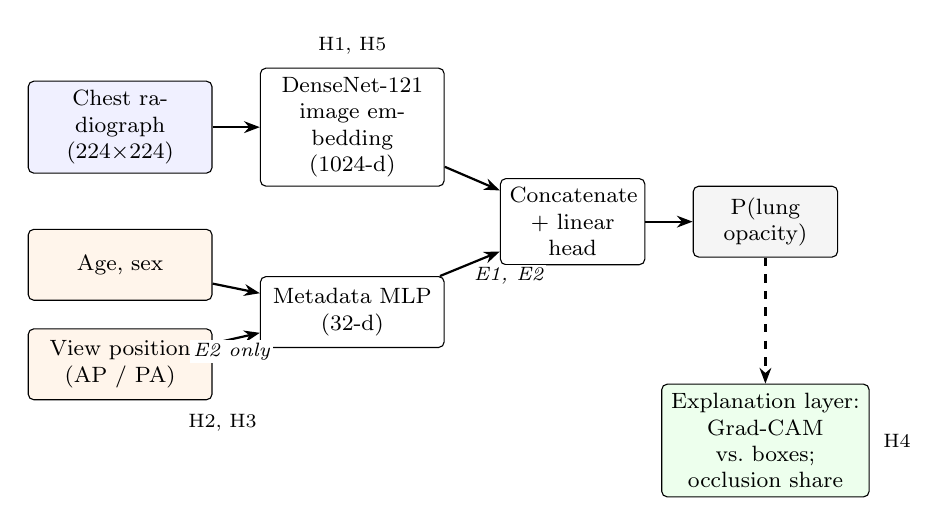
\begin{tikzpicture}[
  font=\footnotesize,
  box/.style={draw, rounded corners=2pt, align=center, minimum height=0.9cm, text width=2.1cm, fill=white},
  inp/.style={box, fill=blue!6},
  meta/.style={box, fill=orange!8},
  xai/.style={box, fill=green!7, text width=2.4cm},
  arr/.style={-{Stealth[length=2mm]}, thick},
  lab/.style={font=\scriptsize\itshape, fill=white, inner sep=1pt}]
\node[inp] (img) {Chest radiograph\\(224$\times$224)};
\node[box, right=0.6cm of img] (cnn) {DenseNet-121\\image embedding\\(1024-d)};
\node[meta, below=0.7cm of img] (as) {Age, sex};
\node[meta, below=0.35cm of as] (view) {View position\\(AP / PA)};
\node[box, right=0.6cm of as, yshift=-0.6cm] (mlp) {Metadata MLP\\(32-d)};
\node[box, right=0.7cm of cnn, yshift=-1.2cm, text width=1.6cm] (fuse) {Concatenate\\+ linear head};
\node[box, right=0.6cm of fuse, text width=1.6cm, fill=gray!8] (out) {P(lung\\opacity)};
\node[xai, below=1.6cm of out] (xai) {Explanation layer:\\Grad-CAM vs.\ boxes;\\occlusion share};
\draw[arr] (img) -- (cnn);
\draw[arr] (as) -- (mlp);
\draw[arr] (view) -- node[lab, below, pos=0.4]{E2 only} (mlp);
\draw[arr] (cnn) -- (fuse);
\draw[arr] (mlp) -- node[lab, below right]{E1, E2} (fuse);
\draw[arr] (fuse) -- (out);
\draw[arr, dashed] (out) -- (xai);
\node[font=\scriptsize, above=0.05cm of cnn] {H1, H5};
\node[font=\scriptsize, below=0.05cm of view, xshift=1.3cm] {H2, H3};
\node[font=\scriptsize, right=0.05cm of xai] {H4};
\end{tikzpicture}}
\caption{Conceptual model. B uses only the image branch; E1 adds age and sex; E2 also adds view position. Hypotheses are attached to the paths they test.}
\label{fig:concept}
\end{figure}

\subsection{Research design}
The study is a quantitative, experimental comparison on secondary data (Fig.~\ref{fig:flow}). All models share data, split, architecture, optimiser and training budget, so the only manipulated factor is the set of inputs.

\begin{figure*}[!t]
\centering
\resizebox{\textwidth}{!}{%
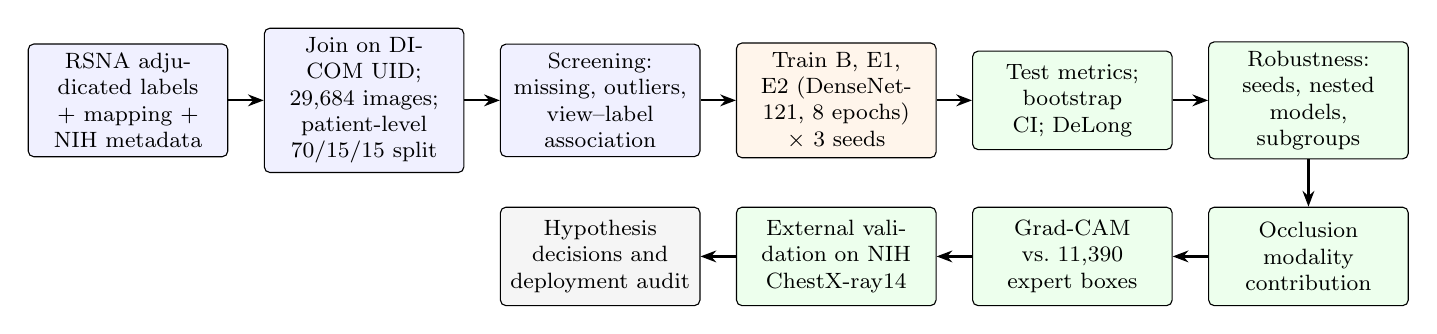
\begin{tikzpicture}[
  font=\footnotesize, node distance=0.45cm,
  stage/.style={draw, rounded corners=2pt, align=center, text width=2.3cm, minimum height=1.25cm, fill=white},
  data/.style={stage, fill=blue!6}, model/.style={stage, fill=orange!8}, eval/.style={stage, fill=green!7},
  arr/.style={-{Stealth[length=2mm]}, thick}]
\node[data] (s1) {RSNA adjudicated labels + mapping + NIH metadata};
\node[data, right=of s1] (s2) {Join on DICOM UID; 29,684 images; patient-level 70/15/15 split};
\node[data, right=of s2] (s3) {Screening: missing, outliers, view--label association};
\node[model, right=of s3] (s4) {Train B, E1, E2 (DenseNet-121, 8 epochs) $\times$ 3 seeds};
\node[eval, right=of s4] (s5) {Test metrics; bootstrap CI; DeLong};
\node[eval, right=of s5] (s6) {Robustness: seeds, nested models, subgroups};
\node[eval, below=0.6cm of s6] (s7) {Occlusion modality contribution};
\node[eval, left=of s7] (s8) {Grad-CAM vs.\ 11,390 expert boxes};
\node[eval, left=of s8] (s9) {External validation on NIH ChestX-ray14};
\node[stage, left=of s9, fill=gray!8] (s10) {Hypothesis decisions and deployment audit};
\draw[arr] (s1) -- (s2); \draw[arr] (s2) -- (s3); \draw[arr] (s3) -- (s4); \draw[arr] (s4) -- (s5);
\draw[arr] (s5) -- (s6); \draw[arr] (s6) -- (s7); \draw[arr] (s7) -- (s8); \draw[arr] (s8) -- (s9); \draw[arr] (s9) -- (s10);
\end{tikzpicture}}
\caption{Research-design flowchart. Blue: data preparation; orange: model training; green: evaluation.}
\label{fig:flow}
\end{figure*}

\subsection{Network architecture}
Fig.~\ref{fig:arch} details the network. The image branch is a DenseNet-121~\cite{huang2017densenet} initialised with ImageNet weights. Its four dense blocks (6, 12, 24 and 16 layers, growth rate 32) are separated by transition layers that halve the spatial size, so a $224\times224$ input yields a $7\times7\times1024$ feature map $A$ after the final batch normalisation. Global average pooling of $\mathrm{ReLU}(A)$ gives the 1024-d image embedding. The metadata branch is a two-layer perceptron that maps the $k$ metadata values to a 32-d embedding. The two embeddings are concatenated (intermediate, feature-level fusion) and passed through dropout and a single linear unit. Grad-CAM reads the gradients at $A$, and the occlusion analysis replaces one input at a time with a neutral value; both act on the trained model without changing it. The base model B uses the same network without the metadata branch.

\begin{figure*}[!t]
\centering
\resizebox{\textwidth}{!}{%
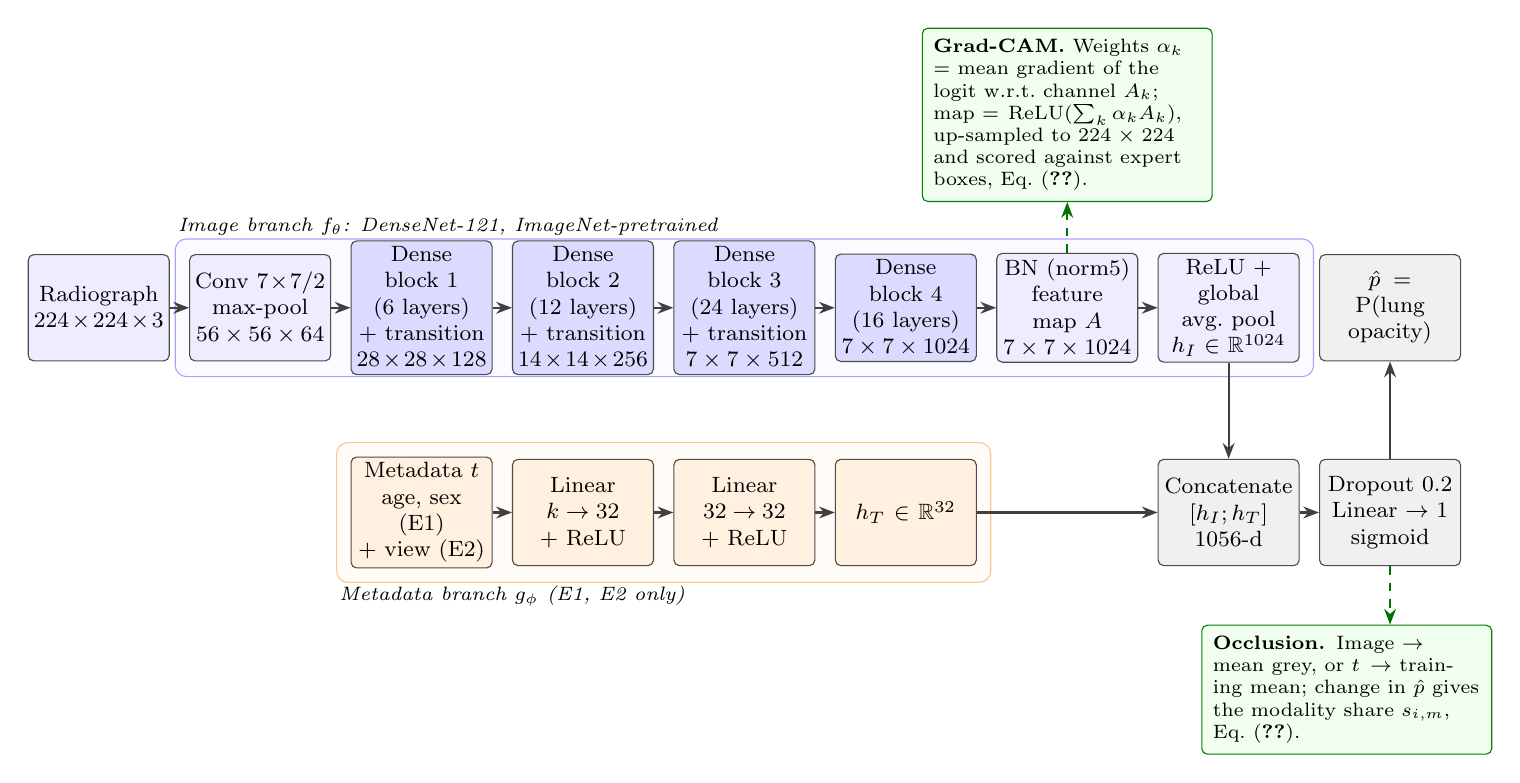
\begin{tikzpicture}[font=\footnotesize,
  blk/.style={draw=black!70, rounded corners=2pt, align=center, text width=1.65cm, minimum height=1.35cm, fill=white, inner sep=2pt},
  img/.style={blk, fill=blue!7},
  den/.style={blk, fill=blue!14},
  met/.style={blk, fill=orange!12},
  fus/.style={blk, fill=gray!12},
  xai/.style={draw=green!50!black, rounded corners=2pt, align=left, text width=3.4cm, fill=green!6, inner sep=4pt, font=\scriptsize},
  arr/.style={-{Stealth[length=2mm]}, thick, black!75},
  xarr/.style={-{Stealth[length=2mm]}, thick, dashed, green!45!black}]
% ----- image branch (row 1)
\node[img] (inp)  at (0,0)     {Radiograph\\$224\times224\times3$};
\node[img] (stem) at (2.05,0)  {Conv $7\times7$/2\\max-pool\\$56\times56\times64$};
\node[den] (d1)   at (4.10,0)  {Dense block 1\\(6 layers)\\+ transition\\$28\times28\times128$};
\node[den] (d2)   at (6.15,0)  {Dense block 2\\(12 layers)\\+ transition\\$14\times14\times256$};
\node[den] (d3)   at (8.20,0)  {Dense block 3\\(24 layers)\\+ transition\\$7\times7\times512$};
\node[den] (d4)   at (10.25,0) {Dense block 4\\(16 layers)\\$7\times7\times1024$};
\node[img] (fm)   at (12.30,0) {BN (norm5)\\feature map $A$\\$7\times7\times1024$};
\node[img] (gap)  at (14.35,0) {ReLU + global\\avg.\ pool\\$h_I\in\mathbb{R}^{1024}$};
\node[fus] (out)  at (16.40,0) {$\hat p=$\\P(lung opacity)};
% ----- metadata branch (row 2)
\node[met] (t)    at (4.10,-2.6)  {Metadata $t$\\age, sex (E1)\\+ view (E2)};
\node[met] (l1)   at (6.15,-2.6)  {Linear $k\!\to\!32$\\+ ReLU};
\node[met] (l2)   at (8.20,-2.6)  {Linear $32\!\to\!32$\\+ ReLU};
\node[met] (ht)   at (10.25,-2.6) {$h_T\in\mathbb{R}^{32}$};
% ----- fusion head (row 2, right)
\node[fus] (cat)  at (14.35,-2.6) {Concatenate\\$[h_I;h_T]$\\1056-d};
\node[fus] (head) at (16.40,-2.6) {Dropout 0.2\\Linear $\to1$\\sigmoid};
% ----- explanation layer
\node[xai] (cam)  at (12.30,2.45) {\textbf{Grad-CAM.} Weights $\alpha_k$ = mean gradient of the logit w.r.t.\ channel $A_k$; map $=\mathrm{ReLU}(\sum_k\alpha_kA_k)$, up-sampled to $224\times224$ and scored against expert boxes, Eq.~\eqref{eq:energy}.};
\node[xai] (occ)  at (15.85,-4.85) {\textbf{Occlusion.} Image $\to$ mean grey, or $t\to$ training mean; change in $\hat p$ gives the modality share $s_{i,m}$, Eq.~\eqref{eq:share}.};
% ----- arrows
\draw[arr] (inp) -- (stem); \draw[arr] (stem) -- (d1); \draw[arr] (d1) -- (d2); \draw[arr] (d2) -- (d3);
\draw[arr] (d3) -- (d4); \draw[arr] (d4) -- (fm); \draw[arr] (fm) -- (gap);
\draw[arr] (t) -- (l1); \draw[arr] (l1) -- (l2); \draw[arr] (l2) -- (ht);
\draw[arr] (ht) -- (cat); \draw[arr] (gap) -- (cat); \draw[arr] (cat) -- (head); \draw[arr] (head) -- (out);
\draw[xarr] (fm) -- (cam);
\draw[xarr] (head.south) -- (head.south |- occ.north);
% ----- group backgrounds
\begin{scope}[on background layer]
\node[fit=(stem)(gap), draw=blue!35, fill=blue!2, rounded corners=4pt, inner sep=5pt,
      label={[font=\scriptsize\itshape, anchor=south west, inner sep=1pt]north west:Image branch $f_\theta$: DenseNet-121, ImageNet-pretrained}] {};
\node[fit=(t)(ht), draw=orange!45, fill=orange!3, rounded corners=4pt, inner sep=5pt,
      label={[font=\scriptsize\itshape, anchor=north west, inner sep=1pt]south west:Metadata branch $g_\phi$ (E1, E2 only)}] {};
\end{scope}
\end{tikzpicture}}
\caption{Network architecture of the base model (B, image branch only) and the fusion extensions (E1, E2). Dense blocks are shaded darker; tensor sizes are given as height $\times$ width $\times$ channels. Dashed green arrows mark the two post-hoc explanation methods, which read the trained network without modifying it.}
\label{fig:arch}
\end{figure*}

\subsection{Model equations}
Let $x$ be a radiograph and $t\in\mathbb{R}^k$ the metadata vector ($k=0$ for B, $k=2$ for E1, $k=3$ for E2). The image embedding is $h_I=\mathrm{GAP}(\mathrm{ReLU}(f_\theta(x)))\in\mathbb{R}^{1024}$, where $f_\theta$ is the DenseNet-121 feature extractor and GAP is global average pooling. The metadata embedding is $h_T=g_\phi(t)\in\mathbb{R}^{32}$, a two-layer perceptron. The predicted probability is
\begin{equation}
\hat p=\sigma\!\left(w^\top[h_I;\,h_T]+b\right),
\label{eq:model}
\end{equation}
where $[\cdot;\cdot]$ denotes concatenation and $\sigma$ the logistic function; for B, Eq.~\eqref{eq:model} reduces to $\sigma(w^\top h_I+b)$. Training minimised the class-weighted binary cross-entropy
\begin{equation}
\mathcal{L}=-\frac{1}{N}\sum_{i=1}^{N}\big[\,w_+ y_i\log\hat p_i+(1-y_i)\log(1-\hat p_i)\big],
\label{eq:loss}
\end{equation}
with $w_+$ equal to the ratio of negative to positive training images. Following the base paper's occlusion principle~\cite{gapp2025modality}, the contribution of modality $m$ to image $i$ is the absolute change in output when $m$ is replaced by a neutral value $\bar m$ (a mean-grey image, or the training-set mean of the metadata):
\begin{equation}
c_{i,m}=\big|\hat p(x_i,t_i)-\hat p_{m\leftarrow\bar m}(x_i,t_i)\big|,\qquad
s_{i,m}=\frac{c_{i,m}}{\sum_{m'}c_{i,m'}}.
\label{eq:share}
\end{equation}
For Grad-CAM map $A_i$ and expert-box mask $B_i$, localisation is measured by the energy in the box and the pointing game~\cite{zhang2018excitation}:
\begin{equation}
E_i=\frac{\sum_{u}A_i(u)B_i(u)}{\sum_u A_i(u)},\qquad
P_i=\mathbb{1}\!\left[B_i\big(\arg\max_u A_i(u)\big)=1\right],
\label{eq:energy}
\end{equation}
and chance level for $E_i$ is the box area fraction $|B_i|/|A_i|$. The paired gain of extension E over B is $\Delta=\mathrm{AUC}_E-\mathrm{AUC}_B$, with a 95\% interval from the 2.5th and 97.5th percentiles of $\Delta$ over 5,000 bootstrap resamples drawn \emph{by patient}~\cite{efron1993bootstrap}, and a DeLong test for correlated AUCs~\cite{delong1988auc}.

% ======================================================================
\section{Base vs.\ Extended Model Comparison}
\label{sec:compare}

Table~\ref{tab:basevsext} sets the base model and its extensions side by side.

\begin{table}[!t]
\caption{Base vs.\ extended models}
\label{tab:basevsext}
\centering
\footnotesize
\begin{tabular}{@{}p{1.55cm}p{1.95cm}p{2.0cm}p{2.0cm}@{}}
\toprule
Aspect & Base (B) & Extension E1 & Extension E2 \\
\midrule
Inputs & Image & Image, age, sex & Image, age, sex, view \\
Architecture & DenseNet-121 & B + MLP, feature-level fusion & as E1 \\
Logic & Image evidence only & Adds patient factors not visible on film & Adds a known acquisition shortcut (control) \\
Explanation & Grad-CAM & Grad-CAM + occlusion share~\cite{gapp2025modality} & as E1, + per-feature occlusion \\
Hypotheses & H5 & H1, H4 & H3, H4 \\
\bottomrule
\end{tabular}
\end{table}

% ======================================================================
\section{Data and Analysis Setup}
\label{sec:setup}

\subsection{Data}
The main dataset is the RSNA Pneumonia Detection Challenge release with adjudicated labels~\cite{shih2019rsna}. These images are a subset of NIH ChestX-ray14~\cite{wang2017chestxray8}. We used the challenge's ``Calculated'' label group, which gives each image one final class: Normal (9,790), No Lung Opacity/Not Normal (12,788) or Lung Opacity (7,106). The outcome was Lung Opacity vs.\ the other two classes, the standard RSNA target, and is described as \emph{lung opacity consistent with pneumonia} rather than confirmed pneumonia. The published RSNA-to-NIH mapping linked every image to the 2020 revision of the NIH metadata (age, sex, view); all 29,684 labelled images matched, and a check on 200 random DICOM files confirmed that their internal identifiers equalled the mapped ones. NIH's own ``Pneumonia'' tag was not used as a label, because it agreed poorly with the radiologist labels (only 414 of 7,106 Lung Opacity images carried it).

The split was made by patient (70/15/15), stratified on whether a patient had any positive image, so that no patient appears in two splits. Table~\ref{tab:profile} gives the sample profile.

\begin{table}[!t]
\caption{Sample profile of the RSNA data by split}
\label{tab:profile}
\centering
\footnotesize
\setlength{\tabcolsep}{3pt}
\begin{tabular}{@{}lrrrrrr@{}}
\toprule
Split & Images & Patients & Opacity \% & Age, mean (SD) & Male \% & AP \% \\
\midrule
\inputrows{tables/tab_profile_rows.tex}
\bottomrule
\end{tabular}
\end{table}

The second (external) dataset consisted of NIH ChestX-ray14 images that are not in the RSNA subset and belong to patients absent from the RSNA training and validation splits. Its labels are mined from reports, so they are noisier. We used two definitions: (A) ``Pneumonia'' vs.\ ``No Finding'' and (B) any of Pneumonia, Consolidation or Infiltration vs.\ ``No Finding''.

\subsection{Data screening}
No values were missing for age, sex, view or label. Three images had a recorded age below one year; they were kept, and age was clipped to 0--100 and scaled to $[0,1]$. Classes were imbalanced (about 24\% positive), which was handled through the loss weight $w_+$ in Eq.~\eqref{eq:loss}. View position was strongly associated with the label ($\chi^2$ test, $p<0.001$, Cram\'er's $V=\cramersV$): 77\% of Lung Opacity images were AP, compared with 18\% of Normal images.

\subsection{Analysis configuration}
Table~\ref{tab:config} lists the settings. Python was chosen because the analysis needs a deep-learning library and a scripted, reproducible pipeline~\cite{paszke2019pytorch,pedregosa2011sklearn}.

\begin{table}[!t]
\caption{Analysis configuration}
\label{tab:config}
\centering
\footnotesize
\begin{tabular}{@{}p{2.5cm}p{5.3cm}@{}}
\toprule
Setting & Value \\
\midrule
Sample size & \nTrain\ train / \nVal\ validation / \nTest\ test images \\
Missing data & None in the variables used \\
Image preprocessing & Min--max scaling, resize to 224$\times$224, ImageNet normalisation; random affine augmentation in training \\
Optimiser & AdamW~\cite{loshchilov2019adamw}, learning rate $10^{-4}$, weight decay $10^{-4}$, one-cycle schedule, batch 32, 8 epochs, mixed precision \\
Model selection & Epoch with the best validation AUC (validation AUC peaked at epochs 2--5, then declined) \\
Decision threshold & Maximises F1 on validation; applied unchanged to test \\
Uncertainty & 5,000 patient-level bootstrap resamples; DeLong test \\
Seeds & 42 (primary), 7, 123 \\
Significance level & $\alpha=0.05$, two-sided \\
Software & Python 3, PyTorch, torchvision, scikit-learn, SciPy on a Kaggle NVIDIA T4 GPU \\
\bottomrule
\end{tabular}
\end{table}

Survey-oriented criteria such as Cronbach's $\alpha$, AVE or HTMT do not apply, because no latent constructs are measured with questionnaire items. Sample size was not set by a power analysis: the full public dataset was used, and the precision it gives is reported directly through the confidence intervals. With 1,082 positive and 3,322 negative test images, the half-width of the AUC interval is about 0.016 (Table~\ref{tab:main}).


% ======================================================================
\section{Results and Discussion}
\label{sec:results}

\subsection{Predictive performance (H1--H3)}
Table~\ref{tab:main} and Fig.~\ref{fig:roc} report test performance. The metadata-only model with age and sex was close to chance (AUC \aucTabAS), but adding view position lifted it to \aucTabASV, without any image input. This supports H2: view position carries substantial label information that is not a lung finding.

\begin{table*}[!t]
\caption{Test-set performance on RSNA (primary seed). AUC with 95\% patient-level bootstrap CI; $\Delta$AUC is relative to the image-only base model. Best value among the deep models in bold.}
\label{tab:main}
\centering
\footnotesize
\begin{tabular}{@{}lccccccc@{}}
\toprule
Model & AUC [95\% CI] & Accuracy & Precision & Recall & F1 & $\Delta$AUC [95\% CI] & DeLong $p$ \\
\midrule
\inputrows{tables/tab_main_rows.tex}
\bottomrule
\end{tabular}
\end{table*}

\begin{figure}[!t]
\centering
\figfile{fig_roc_test.pdf}{\columnwidth}
\caption{ROC curves on the RSNA test split. Dashed lines are metadata-only baselines.}
\label{fig:roc}
\end{figure}

The image-only model reached an AUC of \aucImage. Adding age and sex (E1) gave \aucFusAS, a difference of $\dAucFusAS$ with a bootstrap interval of $[\dAucFusASlo, \dAucFusAShi]$ that includes zero (DeLong $p\pFusAS$). Adding view position as well (E2) gave \aucFusASV\ ($\Delta$AUC $\dAucFusASV$, interval $[\dAucFusASVlo, \dAucFusASVhi]$, DeLong $p\pFusASV$). The threshold-based metrics tell the same story: the fusion models traded a little precision for a little recall, and their F1 scores were within 0.008 of the base model. H1 is therefore not supported: age and sex did not improve detection. H3 is supported: once the image is available, the explicit view variable adds nothing. The likely reason is that the image already shows the projection, so the image branch can encode it without help. Fig.~\ref{fig:aucci} compares the internal and external results.

\begin{figure*}[!t]
\centering
\figfile{fig_auc_ci.pdf}{0.85\textwidth}
\caption{AUC with 95\% patient-level bootstrap intervals for all models on the RSNA test split (left) and the external NIH set, definition B (right).}
\label{fig:aucci}
\end{figure*}

\subsection{Modality contribution (H4)}
Occluding the metadata moved the predicted probability very little. Following Eq.~\eqref{eq:share}, metadata accounted for \shareFusAS\% of the total change in E1 and \shareFusASV\% in E2 (Fig.~\ref{fig:share}); in E2 the share was higher for AP films (\shareFusASVap\%) than for PA films (\shareFusASVpa\%). Per-feature occlusion confirmed the picture: removing age, sex or view each changed the predicted probability by at most 0.0013 on average, against about 0.32 for removing the image. Among the metadata inputs, view had the largest effect, and the share was highest on AP films, which is where the shortcut would act; even there it stayed below 2\%. H4 is supported: the fusion network learned to rely almost entirely on the image. This also explains the null result for H1: a model that barely responds to age and sex cannot gain accuracy from them.

\begin{figure}[!t]
\centering
\figfile{fig_modality_share.pdf}{\columnwidth}
\caption{Share of the prediction change attributable to metadata (Eq.~\eqref{eq:share}) by subset of the test set.}
\label{fig:share}
\end{figure}

\subsection{Grad-CAM localisation (H5)}
For the \nLoc\ test images with expert boxes, the image-only model placed \energyImage\ of its Grad-CAM mass inside the boxes, against a chance level of \energyChance, about twice chance; its peak fell inside a box in \pointImage\ of images (Table~\ref{tab:loc}, Fig.~\ref{fig:gradcam}). The difference from chance was significant for all three models (Wilcoxon signed-rank test, $p<0.001$). H5 is supported, but the absolute agreement is modest, in line with saliency benchmarks~\cite{saporta2022saliency,arun2021trustworthiness}. The examples in Fig.~\ref{fig:gradcam} show both behaviours: some maps cover the marked opacity, while others spread over the mediastinum or the upper chest, and the three models can highlight different regions of the same image even though their predictions are almost identical. Part of the gap is technical: the last DenseNet feature map is $7\times7$, so each Grad-CAM cell covers about $32\times32$ pixels and cannot follow the shape of a small opacity. Fusion did not improve localisation (energy 0.230 and 0.239 vs.\ 0.244; pointing game 0.422 and 0.411 vs.\ 0.454), which is consistent with H4: if the metadata barely affects the output, it cannot redirect where the image branch looks.

\begin{table}[!t]
\caption{Grad-CAM localisation against expert boxes (test positives)}
\label{tab:loc}
\centering
\footnotesize
\setlength{\tabcolsep}{2.5pt}
\begin{tabular}{@{}p{2.3cm}rrrrrr@{}}
\toprule
Model & $n$ & Energy & Chance & Ratio & Pointing & $p$ \\
\midrule
\inputrows{tables/tab_loc_rows.tex}
\bottomrule
\end{tabular}
\\[2pt]{\scriptsize $p$: one-sided Wilcoxon signed-rank test of energy in box vs.\ box area fraction.}
\end{table}

\begin{figure*}[!t]
\centering
\figfile{fig_gradcam_examples.pdf}{0.8\textwidth}
\caption{Grad-CAM maps on four random test images with expert boxes (green) for the three deep models.}
\label{fig:gradcam}
\end{figure*}

\subsection{External validation (H6)}
Table~\ref{tab:external} reports the external results (definition A: \extPosA\ positives of \extNA\ images; definition B: \extPosB\ of \extNB). All models lost accuracy outside the training distribution. The image-only AUC fell from \aucImage\ to \extAucAImage\ under definition A and \extAucBImage\ under definition B. Part of this drop is expected, because NIH's report-mined labels are noisier than the adjudicated RSNA labels, and definition B mixes several findings.

The most telling result concerns the shortcut. The view-including metadata model, which reached \aucTabASV\ internally, fell to \extAucATabASV\ (A) and \extAucBTabASV\ (B), close to chance. The link between view and label in the RSNA subset was therefore a property of how that subset was assembled, not a transferable signal, which is exactly why a model should not lean on it.

On the primary seed the fusion models differed from the base model in both directions: E1 was worse under both definitions ($\Delta$AUC $-0.035$ and $-0.019$, DeLong $p=0.003$ and $p<0.001$), while E2 was slightly better under definition B ($+0.012$, $p=0.001$). These differences did not survive the seed study. Averaged over three seeds, the external AUCs of B, E1 and E2 were 0.765, 0.759 and 0.756 under definition A, and 0.665, 0.664 and 0.666 under definition B. H6 is therefore only partly supported: no fusion model was consistently better or worse than the image-only model, so the internal null result carries over, but single-seed external comparisons are unreliable. Definition A also had only \extPosA\ positives, so its intervals are wide.

\begin{table}[!t]
\caption{External validation on NIH ChestX-ray14 (primary seed)}
\label{tab:external}
\centering
\footnotesize
\setlength{\tabcolsep}{2.5pt}
\begin{tabular}{@{}lp{2.5cm}rcrr@{}}
\toprule
Def. & Model & Pos./$n$ & AUC [95\% CI] & $\Delta$AUC & $p$ \\
\midrule
\inputrows{tables/tab_external_rows.tex}
\bottomrule
\end{tabular}
\end{table}

\subsection{Hypothesis summary}
Table~\ref{tab:hyp} summarises the decisions.

\begin{table}[!t]
\caption{Hypothesis results}
\label{tab:hyp}
\centering
\footnotesize
\begin{tabular}{@{}lp{4.2cm}p{2.4cm}@{}}
\toprule
H & Statement (short) & Result \\
\midrule
H1 & E1 (age, sex) beats B on AUC & Not supported \\
H2 & View lifts metadata-only AUC & Supported (internally only) \\
H3 & View adds nothing to E1 & Supported \\
H4 & Image share above 90\% & Supported \\
H5 & Grad-CAM energy above chance & Supported \\
H6 & Ranking holds externally & Partly (no consistent ranking) \\
\bottomrule
\end{tabular}
\end{table}

% ======================================================================
\section{Robustness Analysis}
\label{sec:robust}

\subsection{Nested models and seeds}
The nested design is itself a component-removal test: E2 $\rightarrow$ E1 removes view, and E1 $\rightarrow$ B removes age and sex. To separate a real effect from training noise, every model was retrained with three seeds (Table~\ref{tab:seeds}, Fig.~\ref{fig:seeds}). Across seeds the mean difference between E1 and B was $\seedDAucFusAS$ (SD \seedDAucFusASsd), and between E2 and B $\seedDAucFusASV$ (SD \seedDAucFusASVsd). Each extension reached DeLong $p<0.05$ in only \seedSigFusAS\ of 3 seeds, and not in the same direction: E1 was significantly better than B with seed 7 ($+0.004$, $p=0.025$), whereas E2 was significantly worse with seed 123 ($-0.005$, $p=0.002$). The seed-to-seed spread was larger than the mean effect. The base model itself was very stable across seeds (AUC SD below 0.001). Removing age and sex, or view, therefore changes performance by less than ordinary training noise, which confirms the null result for H1 and H3.

\begin{table}[!t]
\caption{Seed robustness: test AUC per seed, mean $\pm$ SD, mean gain over B, and number of seeds with DeLong $p<0.05$}
\label{tab:seeds}
\centering
\footnotesize
\setlength{\tabcolsep}{2.5pt}
\begin{tabular}{@{}p{2.2cm}cccccc@{}}
\toprule
Model & s42 & s7 & s123 & Mean $\pm$ SD & $\Delta$ mean & Sig. \\
\midrule
\inputrows{tables/tab_seed_rows.tex}
\bottomrule
\end{tabular}
\end{table}

\begin{figure}[!t]
\centering
\figfile{fig_robust_seeds.pdf}{\columnwidth}
\caption{AUC gain of each extension over the image-only base model for each training seed; the bar marks the mean.}
\label{fig:seeds}
\end{figure}

\subsection{Subgroups (alternative specification)}
Table~\ref{tab:sub} and Fig.~\ref{fig:sub} report AUC within view, sex and age strata. Within AP and within PA films, all deep models scored lower (0.838--0.858) than on the pooled test set (\aucFusASV--\aucImage). Part of the pooled AUC therefore comes from separating AP from PA films, which differ sharply in prevalence (41.7\% vs.\ 10.0\% positive). The image-only model benefits from this as well, because projection is visible on the film. Within each view, the metadata-only models were close to chance (0.51--0.59), which confirms that their apparent skill came from view alone. Performance was similar for women and men, but lower for patients aged 60 or over (about 0.84) than for younger patients (about 0.90), where fusion with age did not close the gap. In no subgroup did a fusion model beat the base model by more than 0.005.

\begin{table}[!t]
\caption{Subgroup AUC on the RSNA test split}
\label{tab:sub}
\centering
\footnotesize
\setlength{\tabcolsep}{2pt}
\begin{tabular}{@{}llrrccccc@{}}
\toprule
 & Level & $n$ & Pos.\% & M-AS & M-ASV & B & E1 & E2 \\
\midrule
\inputrows{tables/tab_subgroup_rows.tex}
\bottomrule
\end{tabular}
\\[2pt]{\scriptsize M-AS/M-ASV: metadata-only models without/with view.}
\end{table}

\begin{figure*}[!t]
\centering
\figfile{fig_subgroups.pdf}{0.85\textwidth}
\caption{Subgroup AUC for the base and extended models; the dashed line is the pooled AUC of the base model.}
\label{fig:sub}
\end{figure*}

% ======================================================================
\section{Practical Implications and Case Study}
\label{sec:case}

Consider a tertiary-care hospital radiology department that is evaluating a commercial ``multimodal'' pneumonia triage tool to prioritise its overnight worklist. Most overnight studies are portable AP films from the emergency department and wards, so the case mix differs from the vendor's validation data. Fig.~\ref{fig:case} shows how the audit developed here would support the procurement decision.

\begin{figure}[!t]
\centering
\resizebox{\columnwidth}{!}{%
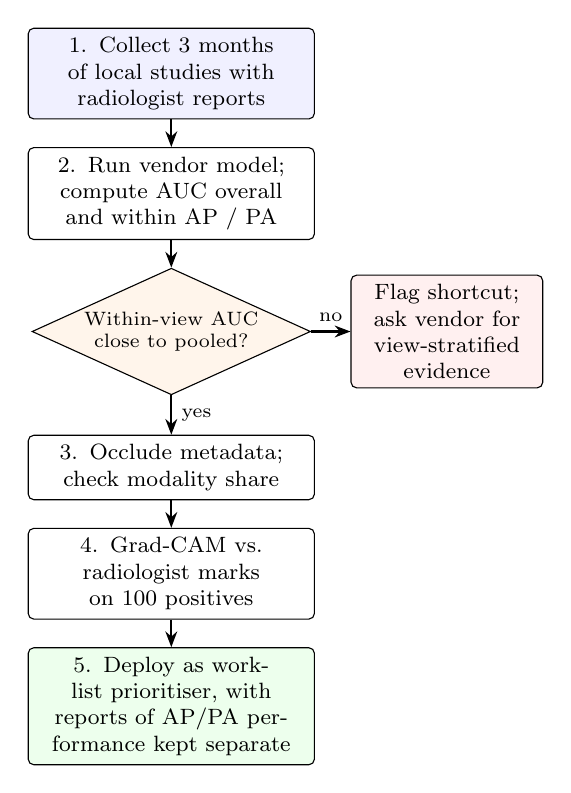
\begin{tikzpicture}[font=\footnotesize, node distance=0.35cm,
  st/.style={draw, rounded corners=2pt, align=center, text width=3.4cm, minimum height=0.8cm, fill=white},
  dec/.style={draw, diamond, aspect=2.2, align=center, inner sep=1pt, fill=orange!8, font=\scriptsize},
  arr/.style={-{Stealth[length=2mm]}, thick}]
\node[st, fill=blue!6] (a) {1. Collect 3 months of local studies with radiologist reports};
\node[st, below=of a] (b) {2. Run vendor model; compute AUC overall and within AP / PA};
\node[dec, below=of b] (c) {Within-view AUC\\close to pooled?};
\node[st, below=0.5cm of c] (d) {3. Occlude metadata; check modality share};
\node[st, right=0.5cm of c, text width=2.2cm, fill=red!6] (r) {Flag shortcut; ask vendor for view-stratified evidence};
\node[st, below=of d] (e) {4. Grad-CAM vs.\ radiologist marks on 100 positives};
\node[st, below=of e, fill=green!7] (f) {5. Deploy as worklist prioritiser, with reports of AP/PA performance kept separate};
\draw[arr] (a) -- (b); \draw[arr] (b) -- (c);
\draw[arr] (c) -- node[right, font=\scriptsize]{yes} (d);
\draw[arr] (c) -- node[above, font=\scriptsize]{no} (r);
\draw[arr] (d) -- (e); \draw[arr] (e) -- (f);
\end{tikzpicture}}
\caption{Case study: a deployment audit for a pneumonia triage tool in a hospital radiology department.}
\label{fig:case}
\end{figure}

\textit{Step 1.} The department assembles a local evaluation set, labelled from final radiologist reports. \textit{Step 2.} It computes AUC on the pooled set and separately for AP and PA films. Our results show why this matters: pooled AUC overstates performance when the two views differ in prevalence, and on an overnight list made mostly of AP films the relevant figure is the within-AP AUC (about 0.84 in our models rather than 0.88). \textit{Step 3.} If the tool accepts patient data, the department occludes each input and checks the modality share; a tool whose output moves strongly with view or ward of origin is likely exploiting the case mix. \textit{Step 4.} Grad-CAM maps are compared with radiologist marks on a sample of positives, using the energy-in-box measure; maps that mostly highlight devices or text markers indicate shortcuts~\cite{degrave2021shortcuts}. \textit{Step 5.} The tool is deployed only as a prioritiser, not a diagnostic decision, and its AP and PA performance are monitored separately.

For the department's management, the main implication is that vendor claims of improvement from ``adding clinical data'' should be accompanied by a modality-level audit. In our data, adding age, sex and view gave no measurable gain, internally or externally, so the cost of linking a hospital information system to the tool would not be justified on accuracy grounds. The external results add a second lesson: a model that had used view position would have lost most of that advantage on another hospital's case mix.

% ======================================================================
\section{Limitations and Threats to Validity}
\label{sec:limits}

\textit{Construct validity.} The positive class is radiological lung opacity, not clinically confirmed pneumonia. The metadata are limited to age, sex and view, so our results do not show that richer clinical data (vital signs, laboratory values) would be ignored in the same way. The occlusion measure depends on the choice of neutral value; mean-grey images and mean metadata are common choices but not the only ones. \textit{Internal validity.} Training on a GPU is not fully deterministic, which is why three seeds were run; three seeds still give only a rough estimate of variance. \textit{External validity.} Both datasets come from one institution (the NIH Clinical Center), and the external labels are report-mined and noisier; the pneumonia-only definition had just 145 positives. \textit{Conclusion validity.} The image-level DeLong test ignores repeated images per patient; the patient-level bootstrap is therefore the primary inference.

Compared with our proposal, two changes were made. The planned MIMIC-based dataset was replaced by RSNA and NIH data, because credentialed access could not be obtained within the project timeline, and because the RSNA expert boxes allow Grad-CAM to be checked against ground truth. The three 2025 comparison studies~\cite{kim2025layerwise,truong2025multimodal,gapp2025modality} use different datasets, so they are compared qualitatively (Table~\ref{tab:lit}) rather than rerun.

% ======================================================================
\section{Conclusion and Future Work}
\label{sec:concl}

We audited whether patient metadata help a pneumonia detector, using nested fusion models and the occlusion-based modality-contribution measure of our base paper. View position was a strong shortcut for a model without the image, but it did not transfer to external data. Once the image was present, neither view nor age and sex changed predictions meaningfully (1--2\% of the prediction change), and fusion gave no reliable gain across seeds or datasets. Grad-CAM agreed with expert boxes about twice as often as chance, but far from perfectly. These findings show that fusing basic demographics with a radiograph should not be assumed to help, and that single-seed comparisons can suggest gains or losses that disappear on replication. Pairing modality contribution with shortcut controls, seed replication and annotated localisation makes such claims testable. Future work should repeat the audit with richer clinical variables, multi-site data and higher-resolution explanation methods, and test with clinicians whether a modality-level explanation changes how much they rely on the model.

% ======================================================================
\section{Compliance with Ethical Standards}
\label{sec:ethics}
This research study was conducted retrospectively using human subject data made available in open access by the National Institutes of Health Clinical Center (ChestX-ray14)~\cite{wang2017chestxray8} and the Radiological Society of North America (RSNA Pneumonia Detection Challenge)~\cite{shih2019rsna}. Ethical approval was not required, as confirmed by the licences attached with the open-access data. All images and metadata were de-identified by the data providers; no attempt was made to re-identify patients. The analysis code, the prepared label table and the codebook are provided with this paper.
\url{https://github.com/Fatima-Siddiqa/explainable-multimodal-pneumonia}.

\section*{Contribution Statement}
% EDIT so it matches what each member actually did.
\textbf{Fatima Siddiqa:} Conceptualisation, Literature review, Writing -- original draft, Visualisation. \textbf{Mariam Shaiq:} Methodology, Software, Data curation, Formal analysis, Writing -- review and editing.

\section*{Acknowledgment}
No funding was received for conducting this study. The authors have no relevant financial or non-financial interests to disclose. Generative AI (Claude, Anthropic) was used to help debug the analysis code and the latex source code. All analyses were run by the authors, and all text, numbers and references were checked by the authors.
\bibliographystyle{IEEEtran}
\bibliography{references}

\end{document}
